%%%%%% CMB-S4 Simulations and Data Analysis Chapter, Forecasting Section  %%%%%%%%%%%%%%%%

\section{Forecasting}

Here we describe the main approaches used by our community for forecasting the expected performance of CMB-S4. For assessing the expected performance for large-scale B-modes, two central considerations are Galactic foregrounds and ability to delens the data, as well as a realistic assessment of instrument noise at large scales. 

To assess the science return from the smaller-scale polarization two-point functions (TE,EE), and from the lensing four-point function ($\kappa \kappa$), extragalactic foregrounds and instrumental noise are the key considerations.

To forecast the return of the thermal Sunyaev-Zel'dovich effects, an estimate of the expected cluster counts as a function of mass and redshift is the core statistic, combined with an estimate of how well the masses can be calibrated using overlaps with weak lensing surveys. For the kinetic Sunyaev-Zeldovich effect, extragalactic foregrounds and overlap with spectroscopic surveys must all be considered. 

\begin{figure}[htbp]
\centering
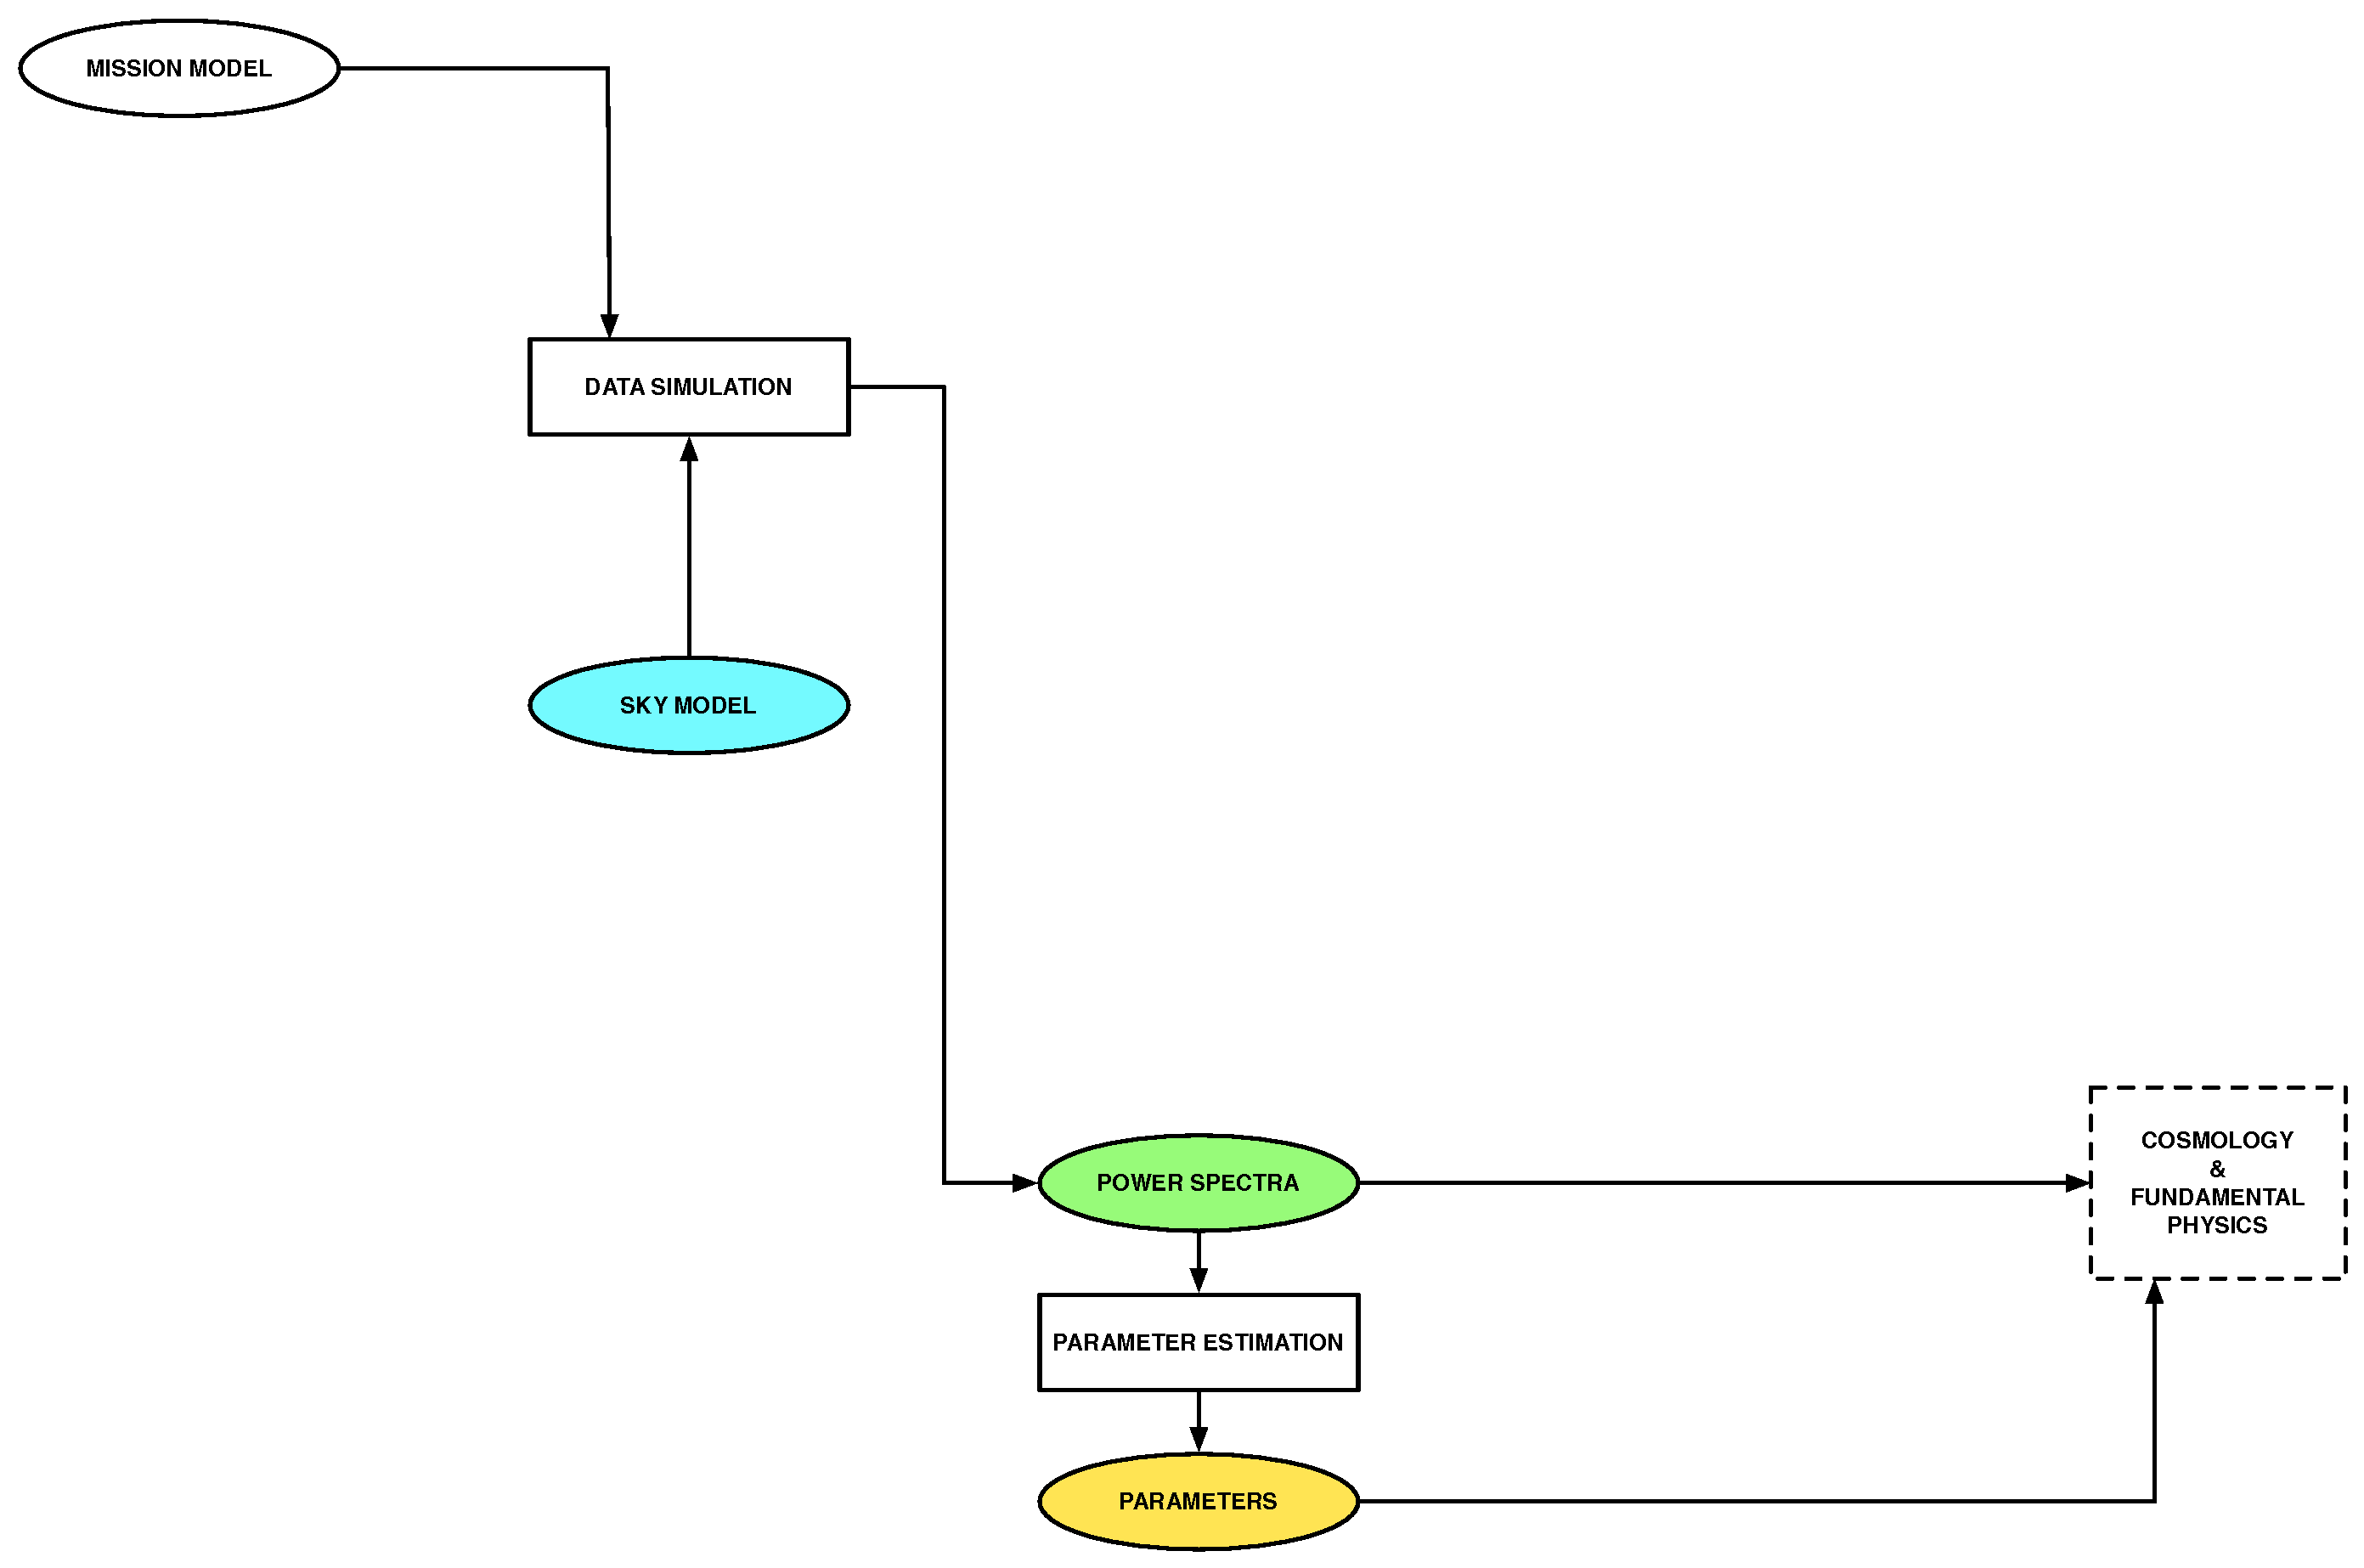
\includegraphics[width=1\textwidth]{Analysis/fc}
\caption{The forecasting subset of the CMB simulation and data analysis pipeline}
\label{default}
\end{figure}


\subsection{Limits on the tensor-to-scalar ratio}

\subsubsection{Spectrum-based domain forecasting}
{\bf Forecasting in spectral domain coming from John Kovac}

\subsubsection{Map-based domain forecasting}

Foregrounds are intrinsically non-Gaussian, so it is beneficial to consider approaches directly in map space, to check the robustness of spectrum-based approaches, in particular in the case of pessimistic foregrounds where the spectral indices or dust emissivities have non-trivial spatial variation. Here one of the approaches our community uses is a Bayesian model fitting method, where the foregrounds are described parametrically using a physical model for each component.

Using this method, maps of the CMB plus Galactic foreground sky and expected noise are simulated at each of the CMB-S4 frequencies and integrated across the expected bandpasses, using Galactic models as described for example in Section \ref{sec:models}. Simulations at ancillary frequencies that might be provided by other experiments, for example the Planck data, can also be included in the same way. A parameterized model is then fit to the simulated maps, for example fitting the CMB, thermal dust, and synchrotron in small pixels, and typically the synchrotron spectral index and dust emissivity and temperature in larger pixels of order degree-scale or larger. The BB power spectrum of the foreground-marginalized CMB map is then estimated using e.g., the Master algorithm or a pixel-based likelihood, and converted into an estimate of $r$ and its uncertainty. Our community has at least two such codes that can perform this procedure (Commander and BFoRe).

This method allows for an assessment of the expected bias on $r$ if the model does not match the simulation, and shows how much the expected uncertainty on $r$ would increase if more complicated foreground models are explored e.g. \cite{armitage-caplan/etal:2011,ramazeilles/etal:2015}. It is more computationally expensive than spectral-domain forecasts though, so we limit this approach to a smaller subset of explorations. 

\subsection{Limits on parameters from TT/TE/EE/$\kappa\kappa$}

To forecast the expected constraints on cosmological parameters from TT/TE/EE and $\kappa\kappa$ for CMB-S4, many of our community's codes use a Fisher matrix method, which assumes that the resulting parameter distributions are close to Gaussian.  Some forecasts are performed using full MCMC simulations if the parameters are known to be highly non-Gaussian. 

For CMB-S4, the method we follow is to combine CMB-S4 specifications with other available datasets, for example the data from Planck and expected measurements of Baryon Acoustic Oscillations and other low redshift data. 

For the noise levels of Planck, we assume that a data release including reliable polarization data will have happened before CMB-S4 data is taken, and forecast results that include TE and EE data and also large-scale polarization from HFI at multipoles lower than CMB-S4 is expected to reach. This follows approaches in e.g. \cite{allison/etal:2015}.

Our community uses two approaches to these Fisher forecasts, either considering the unlensed maps and the lensing convergence map as the basic statistics, or the lensed power spectra of those maps together with the reconstructed $\kappa \kappa$ spectrum. In the case of the power spectrum approach, to compute the Fisher matrix for the CMB we use the lensed power spectrum between each pair of fields $X, Y$:
%
\begin{equation}
\label{eqEstimator}
\hat{C}^{XY}_\ell = \frac{1}{2\ell+1}\sum_{m=-\ell}^{m=\ell} x^{*}_{\ell m} y_{\ell m}.
\end{equation}
%
The estimated power spectrum is Gaussian distribution to good approximation at small scales. In this case a full-sky survey has
%
\begin{equation}
-2\ln\mathcal{L}(\boldsymbol{\theta}) = -2\sum_\ell \ln p( \hat{C}_\ell | \boldsymbol{\theta}) \\
=  \sum_\ell  \Big[ (\hat{C}_\ell - C_\ell(\boldsymbol{\theta}) )^\top  \mathbb{C}^{-1}_\ell(\boldsymbol{\theta}) \big(\hat{C}_\ell - C_\ell(\boldsymbol{\theta})) + \ln \det(2 \pi \mathbb{C}_\ell(\boldsymbol{\theta})) \Big]
\end{equation}
%
where $ \hat{C}_\ell = (\hat{C}_\ell^{TT}, \hat{C}_\ell^{TE}, ...) $ contains auto- and cross-spectra and $\mathbb{C}_\ell$ is their covariance matrix. Discarding any parameter dependence in the power spectrum covariance matrix gives
%
\begin{equation}
F_{ij} = \sum_\ell \frac{\partial C^\top_l}{\partial \theta_i} \mathbb{C}^{-1}_\ell \frac{\partial C_l}{\partial \theta_j}.
\end{equation}
%
Here the covariance matrix for the power spectra has elements
%
\begin{equation}
\mathbb{C}(\hat{C}_l^{\alpha \beta}, \hat{C}_l^{\gamma \delta}) = \frac{1}{(2l+1)f_{\rm sky}} \big[ (C_l^{\alpha \gamma} + N_l^{\alpha \gamma}) (C_l^{\beta \delta} + N_l^{\beta \delta})  \\
+ (C_l^{\alpha \delta} + N_l^{\alpha \delta}) (C_l^{\beta \gamma} + N_l^{\beta \gamma}) \big],
\end{equation}
%
where $\alpha, \beta, \gamma, \delta \in \{T, E, B, \kappa_c\}$ and $f_{\rm sky}$ is the effective fractional area of sky used. 

The second approach we consider is to construct the Fisher matrix using the unlensed temperature and polarization fields, and the lensing convergence field, rather than the suite of lensed two-point spectra and the lensing four-point function. Both approaches give consistent estimates.

The CMB lensing reconstruction noise is calculated using the \cite{Hu:2002} quadratic-estimator formalism. Our nominal approach is to neglect non-Gaussian terms in the power spectrum covariance. We also avoid including information from both lensed BB and the four-point $\kappa \kappa$, as they are covariant. The BB spectrum will not contribute as significantly to S4 constraints, compared to $\kappa \kappa$, and has a highly non-Gaussian covariance \cite{Benoit-Levy:2012}. 

To address the issue of possible extragalactic foregrounds, we set a maximum multipole for the recoverable information of $\ell^T_{\rm max} = 3000$ and $\ell^P_{\rm max} = 4000$ for CMB-S4, as foregrounds are expected to be limiting at smaller scales. We also set a minimum multipole due to the challenge of recovering large-scales from the ground, and consider in general $\ell=50$. We include Planck data at the scales $\ell<\ell_{\rm min}$. 

When relevant, we can also add information from Baryon Acoustic Oscillation (BAO) experiments. This can be done by adding the BAO Fisher matrix
%
\begin{equation}
F_{ij}^{\rm BAO} = \sum_{k} \frac{1}{\sigma_{f,k}^2}\frac{\partial f_k}{\partial \theta_i}\frac{\partial f_k}{\partial \theta_j}
\end{equation}
%
where $f_k = r_s/d_V(z_k)$ is the sound horizon at photon-baryon decoupling $r_s$ over the volume distance $d_V$ to the source galaxies at redshift $z_k$. We also follow standard approaches to including other low redshift probes.
%, 

\subsubsection{Instrument and atmospheric noise}
Noise spectra are generated assuming the sum of white noise and atmospheric noise. The white noise part is given by
%
\begin{equation}
N^{\alpha \alpha}_\ell = (\Delta T)^2 \exp \left( \frac{\ell(\ell + 1) \theta^2_{\rm FWHM}}{8 \ln 2} \right)
\end{equation}
%
for $\alpha \in \{T, E, B\}$, where $\Delta T$ ($\Delta P$ for polarization) is the map sensitivity in $\mu$K-arcmin and $\theta_{\rm FWHM}$ is the beam width. 

To estimate the atmospheric noise level in intensity, we consider levels at the South Pole and in Chile. For Chile, we base this estimate on current data from ACT and POLARBEAR. for the South Pole, we use data from SPT and BICEP as a guide. We then make the assumption that the atmospheric noise will scale down with observation time for detector arrays within a telescope, and will be uncorrelated for physically separated telescopes. For polarization our nominal estimate is white noise, assuming that use of modulators minimizes atmospheric contamination.

%

\subsection{Limits on parameters from tSZ/kSZ}

To estimate the expected tSZ cluster counts from S4, we use.
